\documentclass[11pt,a4paper]{article}
\usepackage[T1]{fontenc}
\usepackage[utf8]{inputenc}
\usepackage{lmodern}
\usepackage[spanish,es-nodecimaldot]{babel}
\usepackage[margin=2cm,headheight=15pt]{geometry}
\usepackage{graphicx,array,booktabs,tabularx,xcolor,enumitem,fancyhdr}
\usepackage{hyperref}
\definecolor{azul}{HTML}{173B5E}
\definecolor{gris}{HTML}{EEF3F7}
\hypersetup{colorlinks=true,urlcolor=azul,linkcolor=azul,
 pdftitle={Registro de aplicación y entrega del Client ID},
 pdfauthor={CHC Consultores},pdfsubject={Guía para el administrador de TI}}
\setlength{\parindent}{0pt}
\setlength{\parskip}{6pt}
\setlength{\emergencystretch}{3em}
\setlist[enumerate]{leftmargin=*,itemsep=4pt,topsep=4pt}
\setlist[itemize]{leftmargin=*,itemsep=3pt,topsep=4pt}
\pagestyle{fancy}
\fancyhf{}
\fancyhead[L]{\small\color{azul} Microsoft Entra ID · Guía para TI}
\fancyfoot[L]{\small Registro de aplicación · Octubre de 2026}
\fancyfoot[R]{\small\thepage}
\renewcommand{\headrulewidth}{0.3pt}
\newcommand{\codigo}[1]{\texttt{\detokenize{#1}}}
\newcommand{\titulo}[1]{{\Large\bfseries\color{azul}#1\par}\smallskip}
\newcommand{\nota}[1]{\par\smallskip\colorbox{gris}{\parbox{\dimexpr\linewidth-2\fboxsep}{\small #1}}\par\smallskip}
\newcommand{\pie}[1]{{\small\color{azul}#1\par}}
\graphicspath{{capturas_registro/}{docs/seguridad/capturas_registro/}}

\begin{document}
\titulo{Registro de aplicación y entrega del Client ID}
\textbf{Procedimiento para el administrador de TI de la organización}

Esta guía describe cómo registrar en Microsoft Entra ID la aplicación de
escritorio que descarga el libro de cargas de SharePoint y envía los reportes
mediante Microsoft Graph. El registro debe crearse en el directorio
(\textit{tenant}) de la organización que proporcionará esas cuentas y recursos.
Microsoft genera el \textbf{Client ID} al registrar la aplicación; no es una
contraseña que deba elegir el administrador.

\section*{Naturaleza pública del identificador}
El \textbf{Client ID} identifica la aplicación ante Microsoft y es un valor
público por diseño. Compartirlo con el equipo encargado de configurar el
programa no equivale a entregar una credencial ni concede, por sí solo,
acceso a correos, archivos o funciones administrativas de la empresa.
El acceso continúa sujeto al inicio de sesión del usuario, los permisos
consentidos y las políticas del directorio.

Microsoft lo expresa en su documentación oficial: \textit{«The client ID is
a public value that identifies the application»}. En la misma sección
distingue el \textit{client secret}, que sí es confidencial.

\href{https://learn.microsoft.com/en-us/entra/identity-platform/msal-client-applications\#secrets-and-their-importance-in-proving-identity}{Microsoft Learn: Public client and confidential client applications, sección «Secrets and their importance in proving identity».}

{\small\url{https://learn.microsoft.com/en-us/entra/identity-platform/msal-client-applications}}

El \textbf{Tenant ID} identifica el directorio y también es un dato de
configuración, no una contraseña. Para esta integración se entregan ambos
identificadores. No se requieren \textit{client secrets}, contraseñas,
claves privadas, tokens ni cookies de sesión.

\section*{Antes de comenzar}
\begin{itemize}
\item Utilizar una cuenta autorizada para registrar aplicaciones y conceder
consentimiento. El rol \textbf{Administrador de aplicaciones en la nube}
permite aprobar los permisos delegados de esta guía.
\item Identificar la cuenta operadora: debe disponer de un buzón de
Exchange Online y acceso de lectura al archivo de SharePoint.
\item Tener a mano la URL del sitio y la ruta del libro que utilizará el programa.
\end{itemize}
\href{https://learn.microsoft.com/en-us/entra/identity/enterprise-apps/grant-admin-consent}{Microsoft Learn: roles autorizados y consentimiento administrativo.}

\nota{Las capturas proceden de un registro temporal de demostración,
eliminado al finalizar la documentación. Los nombres y los identificadores
visibles son de ejemplo: utilice los de su organización. Los números señalan
los controles citados en cada paso.}

\newpage
\titulo{1. Abrir el registro de aplicaciones}
\begin{enumerate}
\item Ingresar a \href{https://entra.microsoft.com}{entra.microsoft.com}.
Comprobar en el menú de cuenta que el directorio seleccionado corresponde
a la organización donde se instalará la integración.
\item Buscar \textbf{Registros de aplicaciones} en la barra superior y abrir
el servicio. También puede aparecer bajo \textbf{Entra ID > Aplicaciones}.
\item Seleccionar \textbf{Nuevo registro}, marcado con el número 1.
\end{enumerate}
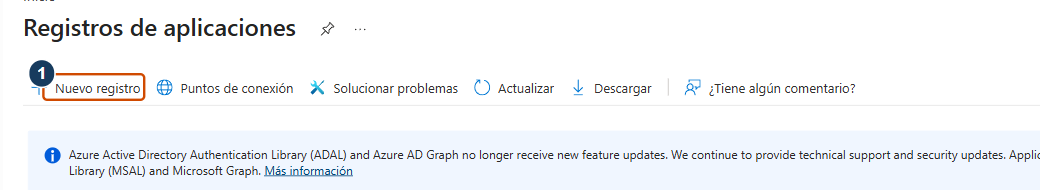
\includegraphics[width=\linewidth]{01_nuevo_registro.png}

\titulo{2. Crear la aplicación de escritorio}
Completar los cinco controles marcados en la captura:
\begin{enumerate}
\item \textbf{Nombre}: usar un nombre identificable, por ejemplo,
\textit{Gestor de reportes}. El sufijo «Ejemplo temporal» es solo de la demostración.
\item \textbf{Tipos de cuenta compatibles}: seleccionar \textbf{Solo las
cuentas de este directorio organizativo} o \textbf{Solo inquilino único}.
Verificar que se indique el nombre de su organización.
\item \textbf{URI de redirección}: elegir \textbf{Cliente público o nativo
(móvil y escritorio)} como plataforma.
\item Escribir exactamente \codigo{http://localhost} como dirección de retorno.
\item Pulsar \textbf{Registrar} y esperar la pantalla de información general.
\end{enumerate}
\begin{center}
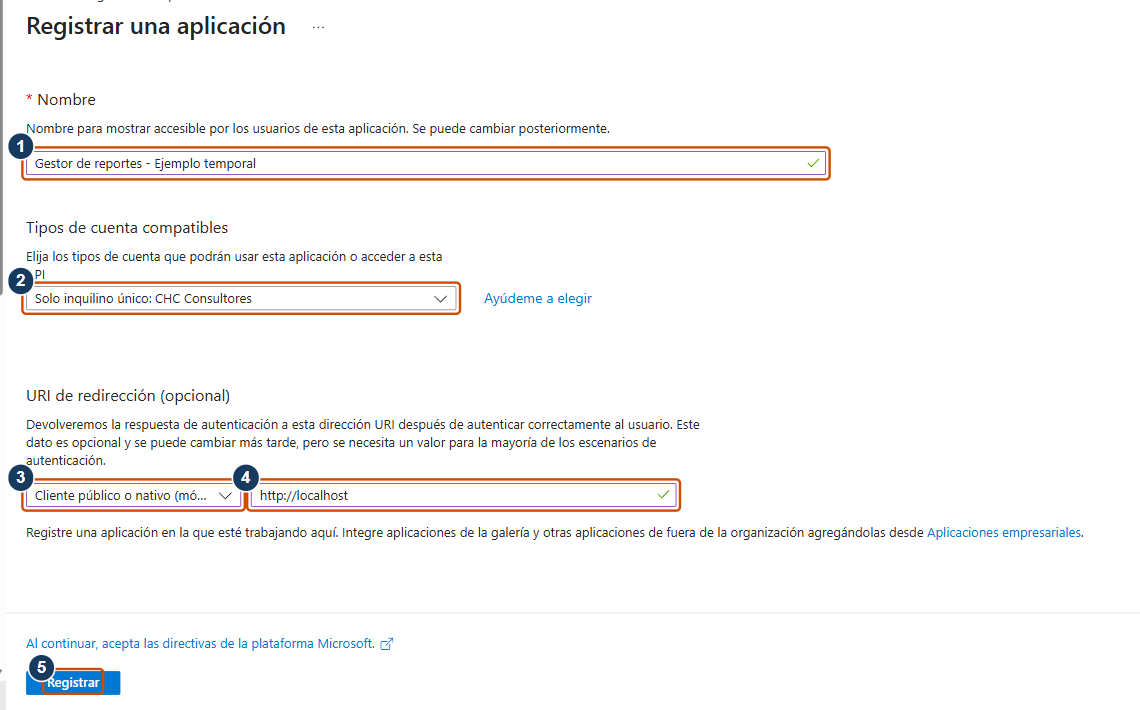
\includegraphics[width=\linewidth,height=9.9cm,keepaspectratio]{02_formulario_registro.png}
\end{center}
\pie{El Client ID se genera automáticamente al completar el registro.}

\newpage
\titulo{3. Verificar la dirección de retorno}
Abrir \textbf{Administrar > Autenticación}; en algunas versiones aparece como
\textbf{Authentication (Preview)} (1). Confirmar que la plataforma
\textbf{Aplicaciones móviles y de escritorio} contenga \codigo{http://localhost} (2).

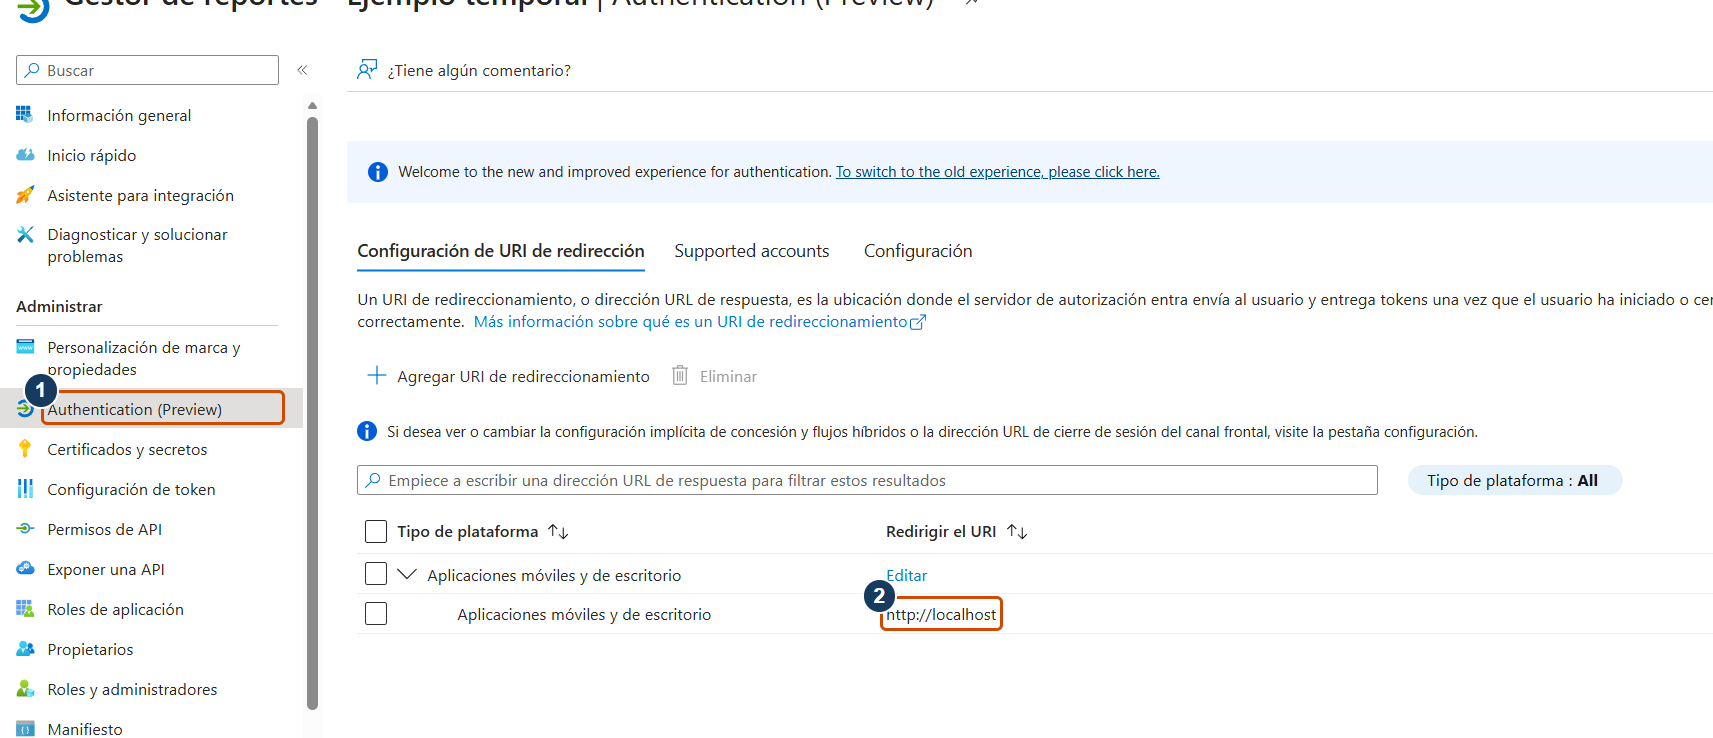
\includegraphics[width=\linewidth,trim=0 0 0 30,clip]{03_redireccion.png}

Si no se agregó durante el registro, seleccionar \textbf{Agregar URI de
redireccionamiento} o \textbf{Agregar una plataforma}; elegir
\textbf{Aplicaciones móviles y de escritorio}, introducir
\codigo{http://localhost} y guardar.

Esta dirección devuelve el inicio de sesión al equipo donde se ejecuta el
programa. El retorno de correo utiliza \codigo{http://localhost:62190/};
Microsoft omite el puerto al comparar las URI de \codigo{localhost}.
\href{https://learn.microsoft.com/en-us/entra/identity-platform/reply-url\#localhost-exceptions}{Referencia oficial: excepciones de localhost.}
No es necesario habilitar la concesión implícita ni crear un secreto para este flujo.

\titulo{4. Abrir los permisos de Microsoft Graph}
Ir a \textbf{Administrar > Permisos de API > Agregar un permiso}.
Seleccionar \textbf{Microsoft Graph} y luego \textbf{Permisos delegados}.

\begin{minipage}[t]{0.48\linewidth}
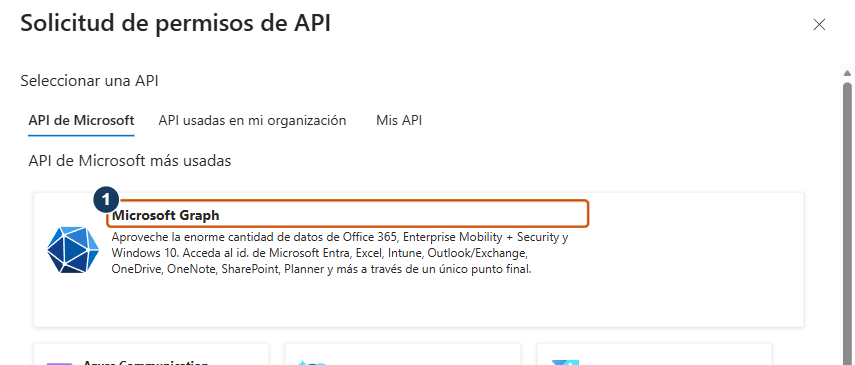
\includegraphics[width=\linewidth]{04_elegir_graph.png}
\pie{A. Seleccionar Microsoft Graph.}
\end{minipage}\hfill
\begin{minipage}[t]{0.48\linewidth}
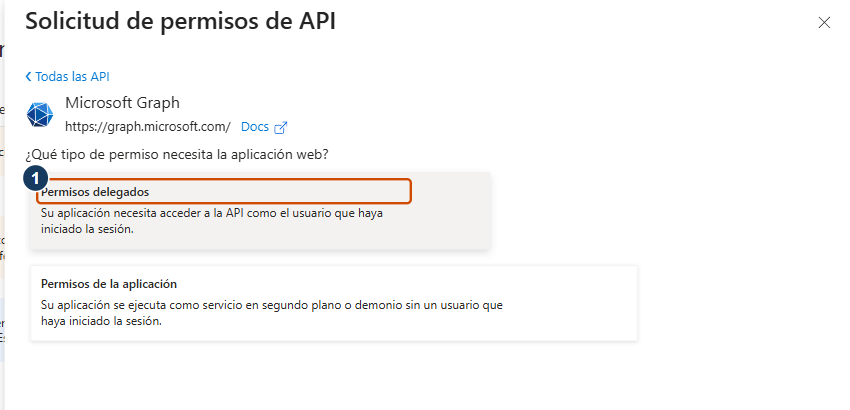
\includegraphics[width=\linewidth,trim=5 0 0 0,clip]{05_tipo_delegado.png}
\pie{B. Seleccionar Permisos delegados.}
\end{minipage}

\nota{Todos los permisos de esta guía son delegados: el programa trabaja
en nombre del usuario que inicia sesión. No seleccionar «Permisos de la aplicación».}

\newpage
\titulo{5. Configurar el envío de correo}
\begin{enumerate}
\item En \textbf{Buscar permisos}, escribir \codigo{Mail.Send} (1).
\item Expandir el grupo \textbf{Mail} con la flecha y marcar
\codigo{Mail.Send}, cuya descripción es \textbf{Enviar correo como usuario} (2).
\item Pulsar \textbf{Agregar permisos} para guardar la selección (3).
\item Verificar que también figure \codigo{User.Read}. Normalmente se agrega
al crear el registro. Si falta, repetir el procedimiento, buscar
\codigo{User.Read}, expandir \textbf{User}, marcarlo y guardar.
\end{enumerate}
\begin{center}
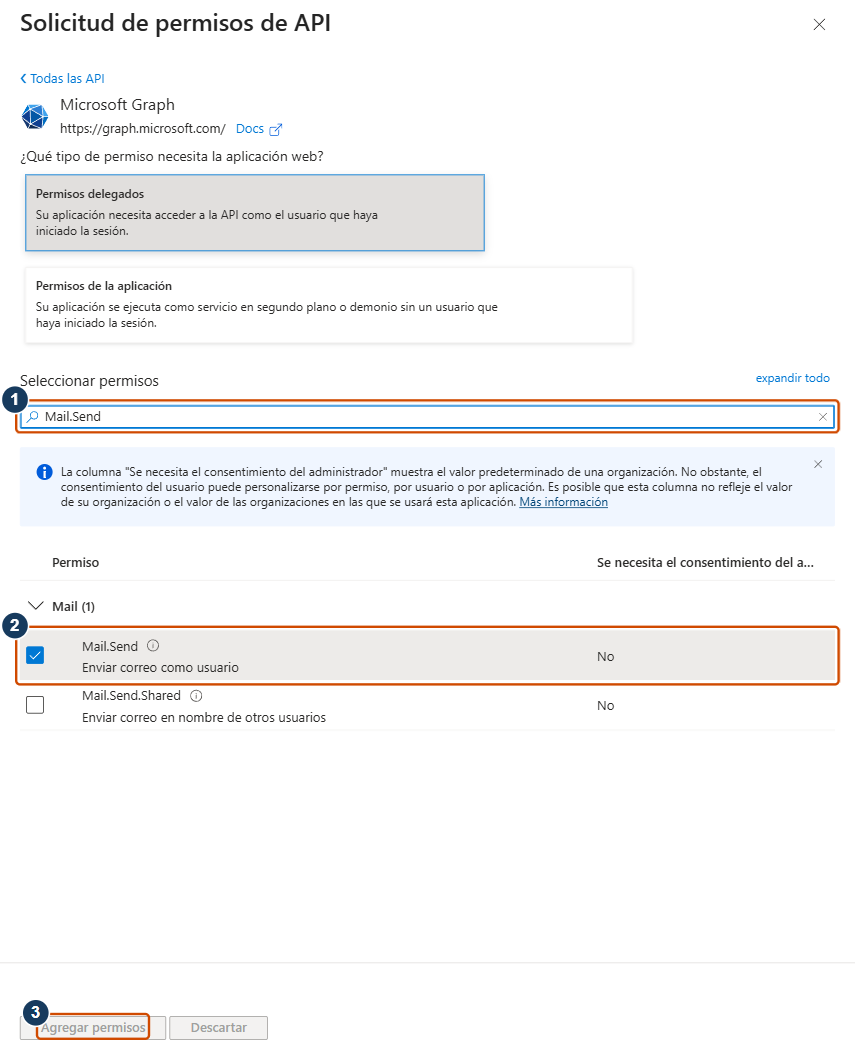
\includegraphics[height=17cm,width=\linewidth,keepaspectratio]{06_mail_send.png}
\end{center}
\pie{1. Búsqueda.\quad 2. Permiso exacto.\quad 3. Guardar la selección.}
{\small En la captura el permiso ya está guardado; por eso «Agregar permisos»
aparece inactivo. Se habilita cuando se añade una selección nueva.}

\newpage
\titulo{6. Configurar la lectura de SharePoint}
\begin{enumerate}
\item Volver a \textbf{Permisos de API > Agregar un permiso} y seleccionar
\textbf{SharePoint}. Si no aparece, abrir \textbf{API usadas en mi organización}
y buscar \textit{SharePoint}.
\item Elegir \textbf{Permisos delegados}. En \textbf{Buscar permisos},
escribir \codigo{AllSites.Read} (1).
\item Expandir \textbf{AllSites}, marcar \codigo{AllSites.Read} (2) y pulsar
\textbf{Agregar permisos} (3).
\end{enumerate}
\begin{center}
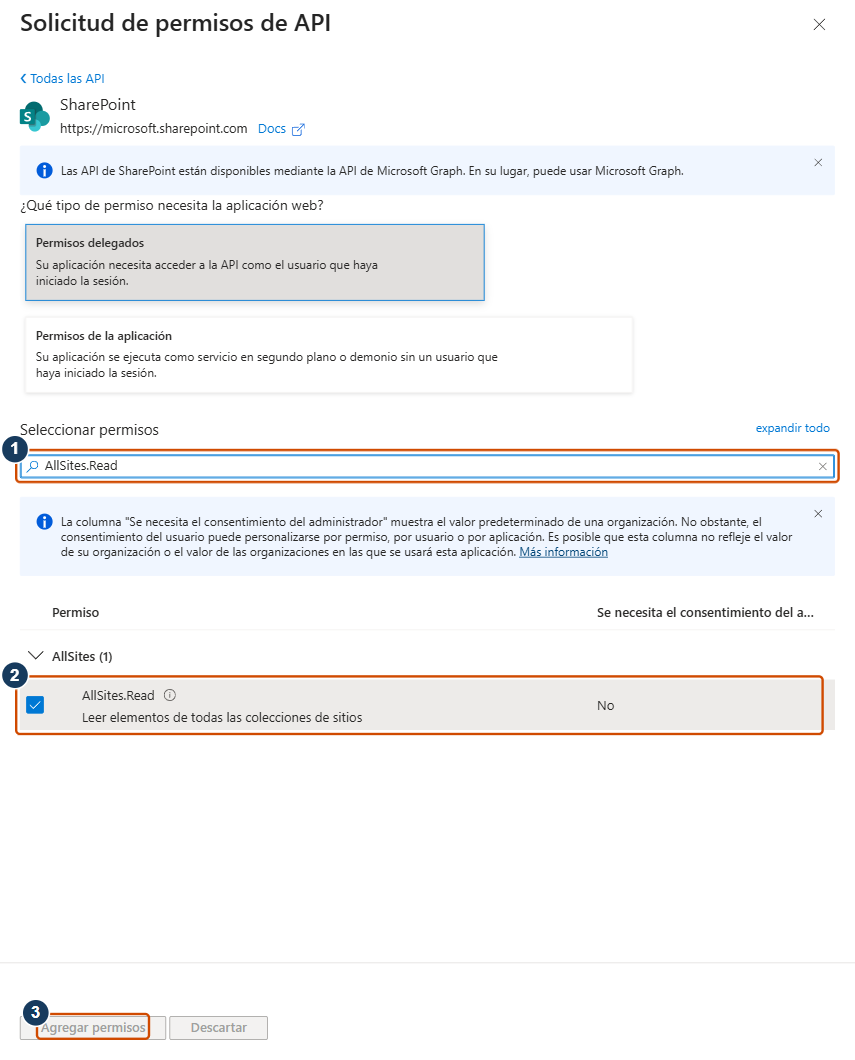
\includegraphics[height=16.5cm,width=\linewidth,keepaspectratio]{07_sharepoint_read.png}
\end{center}
\pie{El permiso pertenece a la API SharePoint, no a Microsoft Graph.}
{\small La captura muestra la selección ya guardada. Este permiso permite
leer sitios a los que tenga acceso el usuario; su alcance no queda limitado
al libro configurado. La aplicación actual descarga el archivo mediante la
API REST de SharePoint.}

\newpage
\titulo{7. Revisar y conceder el consentimiento}
En \textbf{Permisos de API} (1), comprobar esta lista exacta:
\begin{center}
\begin{tabularx}{\linewidth}{@{}lllX@{}}
\toprule
API & Permiso & Tipo & Finalidad \\
\midrule
Microsoft Graph & \codigo{User.Read} & Delegado & Perfil del usuario autenticado. \\
Microsoft Graph & \codigo{Mail.Send} & Delegado & Envío desde su buzón. \\
SharePoint & \codigo{AllSites.Read} & Delegado & Lectura del archivo de cargas. \\
\bottomrule
\end{tabularx}
\end{center}
\begin{enumerate}
\item Seleccionar \textbf{Conceder consentimiento de administrador para
[organización]} (2).
\item Revisar que el cuadro de confirmación corresponda a la aplicación
recién creada y al directorio correcto; confirmar la concesión.
\item Actualizar la página y comprobar que en la columna \textbf{Estado}
de los tres permisos (3) aparezca \textbf{Concedido para [organización]}.
\end{enumerate}
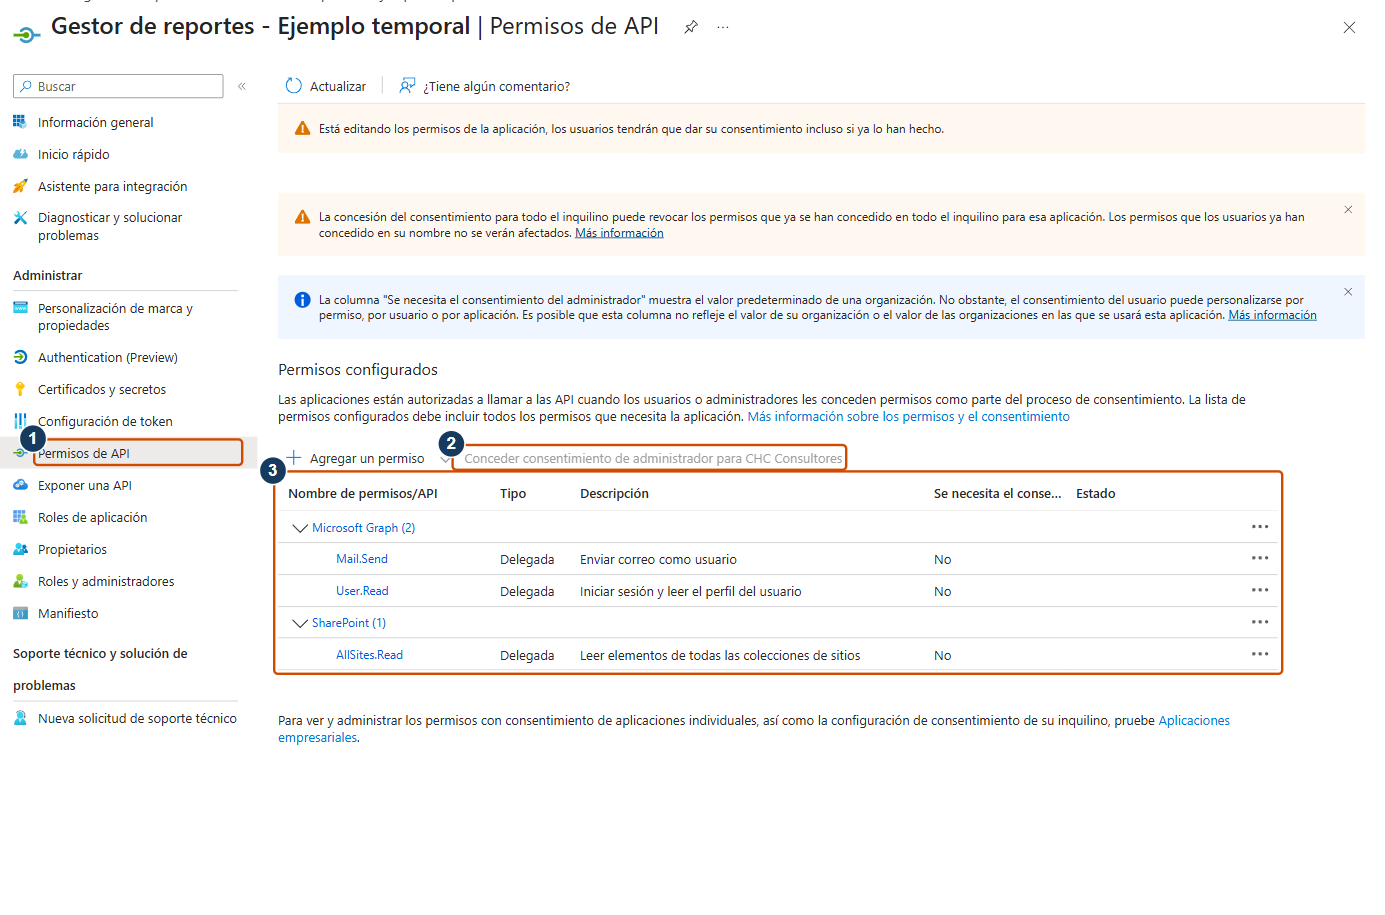
\includegraphics[width=\linewidth]{08_permisos_consentimiento.png}
\nota{La captura muestra los permisos configurados, aún sin consentimiento.
El botón está deshabilitado para la cuenta de demostración. Si ocurre lo
mismo, este paso debe realizarlo una cuenta con un rol autorizado, como
Administrador de aplicaciones en la nube. No es necesario ampliar los permisos de la aplicación.}

La columna \textbf{Se necesita el consentimiento del administrador: No}
no significa que el consentimiento ya se haya concedido. La aprobación
tampoco asigna un buzón, concede acceso al archivo ni evita MFA o las
políticas de acceso condicional.
\href{https://learn.microsoft.com/en-us/entra/identity/enterprise-apps/grant-admin-consent}{Procedimiento oficial de consentimiento administrativo.}

\newpage
\titulo{8. Entregar los datos para configurar el programa}
Volver a \textbf{Información general}. Copiar desde \textbf{Información esencial}:
\begin{enumerate}
\item \textbf{Id. de aplicación (cliente)}: corresponde al \textbf{Client ID}.
\item \textbf{Id. de directorio (inquilino)}: corresponde al \textbf{Tenant ID}.
\end{enumerate}
\begin{center}
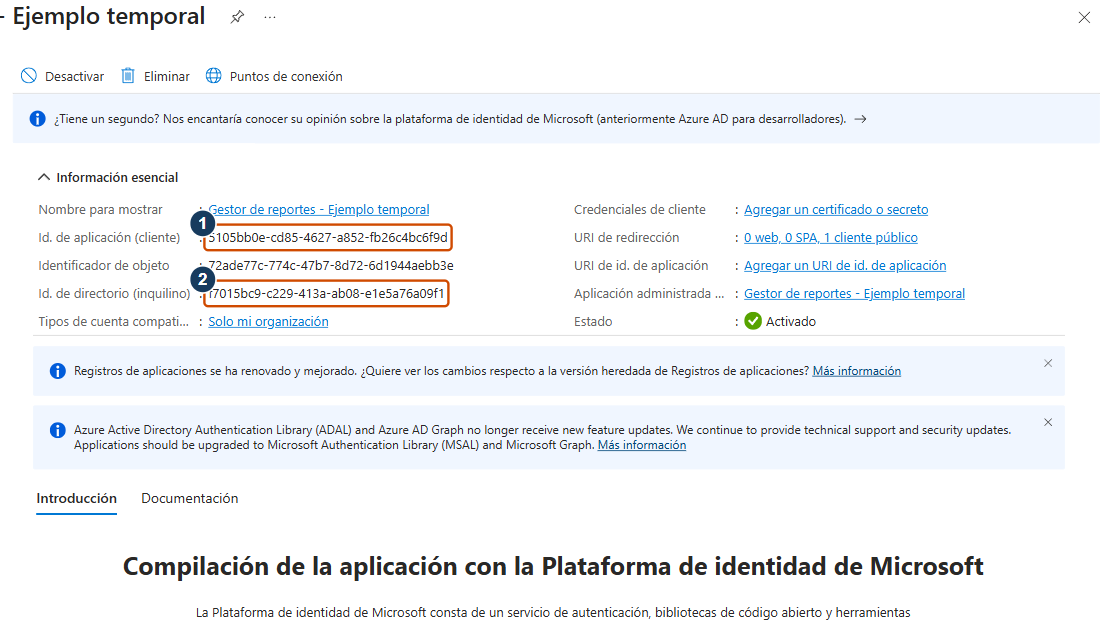
\includegraphics[width=\linewidth,trim=0 278 0 152,clip]{09_identificadores.png}
\end{center}
\pie{Copiar los valores del registro definitivo. No utilizar los identificadores de esta captura.}

\textbf{Información que TI debe entregar al equipo de desarrollo:}
\begin{center}
\begin{tabularx}{\linewidth}{@{}p{4.5cm}X@{}}
\toprule
Dato & Contenido solicitado \\
\midrule
Client ID & Valor completo de «Id. de aplicación (cliente)». \\
Tenant ID & Valor completo de «Id. de directorio (inquilino)». \\
Permisos y consentimiento & Confirmación de los tres permisos delegados y su
estado concedido; preferiblemente una captura de la lista. \\
Redirección & Confirmación de \codigo{http://localhost} en la plataforma de escritorio. \\
Ubicación del libro & URL del sitio y ruta relativa del archivo en SharePoint. \\
Cuenta operadora & Dirección de correo de la cuenta que iniciará sesión y
confirmación de acceso al buzón y al archivo. \\
\bottomrule
\end{tabularx}
\end{center}

\textbf{Ejemplo de ubicación del libro, para sustituir por los datos reales:}

{\small
Sitio: \url{https://empresa.sharepoint.com/sites/Operaciones}\par
Archivo: \codigo{/sites/Operaciones/Documentos compartidos/Informe de cargas Power BI.xlsm}\par}

La ruta del archivo debe ser relativa al servidor y comenzar con
\codigo{/sites/} cuando el sitio use esa estructura. No debe ser únicamente
un enlace de uso compartido. Si el directorio o el sitio tienen otra
estructura, entregar la ruta correspondiente al archivo real.

\nota{No se solicita el «Identificador de objeto», un Client Secret,
contraseñas, tokens ni acceso a la cuenta del administrador. El registro
debe conservarse activo: su eliminación impediría el funcionamiento del programa.}

\textbf{Integración y verificación.} El equipo de desarrollo incorporará el
Client ID y el Tenant ID recibidos y configurará ambas autoridades de
autenticación con esta dirección, sustituyendo el identificador del directorio:
\par{\small\codigo{https://login.microsoftonline.com/<TENANT_ID>}}\par
Después se verificará el inicio de sesión y la lectura del archivo con la
cuenta operadora. Cualquier envío de prueba se coordinará previamente.
\end{document}

